\documentclass[aspectratio=169]{beamer}

% Required packages
\usepackage{physics}
\usepackage{tikz}
\usepackage{amsmath}
\usepackage{graphicx}
\usepackage{xcolor}

% Define custom colors
\definecolor{ds9blue}{RGB}{25,25,112}
\definecolor{ds9gold}{RGB}{218,165,32}
\definecolor{ds9grey}{RGB}{105,105,105}
\definecolor{ds9red}{RGB}{178,34,34}

% Theme configuration
\usetheme{Madrid}
\usecolortheme{whale}
\setbeamercolor{palette primary}{bg=ds9blue,fg=white}
\setbeamercolor{palette secondary}{bg=ds9gold,fg=black}
\setbeamercolor{structure}{fg=ds9blue}

% Title information
\title[Linear Momentum]{PHYS11 CH8: Linear Momentum \& Collisions}
\subtitle{Understanding Motion Through Conservation Laws}
\author[Mr. Gullo]{Mr. Gullo}
\date[]{}

\begin{document}

\frame{\titlepage}

% Learning Objectives
\begin{frame}
\frametitle{Learning Objectives}
\begin{itemize}
\item Define and calculate linear momentum
\item Understand impulse and its relationship to force
\item Apply conservation of momentum in various scenarios
\item Analyze elastic and inelastic collisions
\item Solve problems involving two-dimensional collisions
\item Understand basic rocket propulsion principles
\end{itemize}
\end{frame}
\begin{frame}{Chang’e-5 }
    \begin{figure}
        \centering
        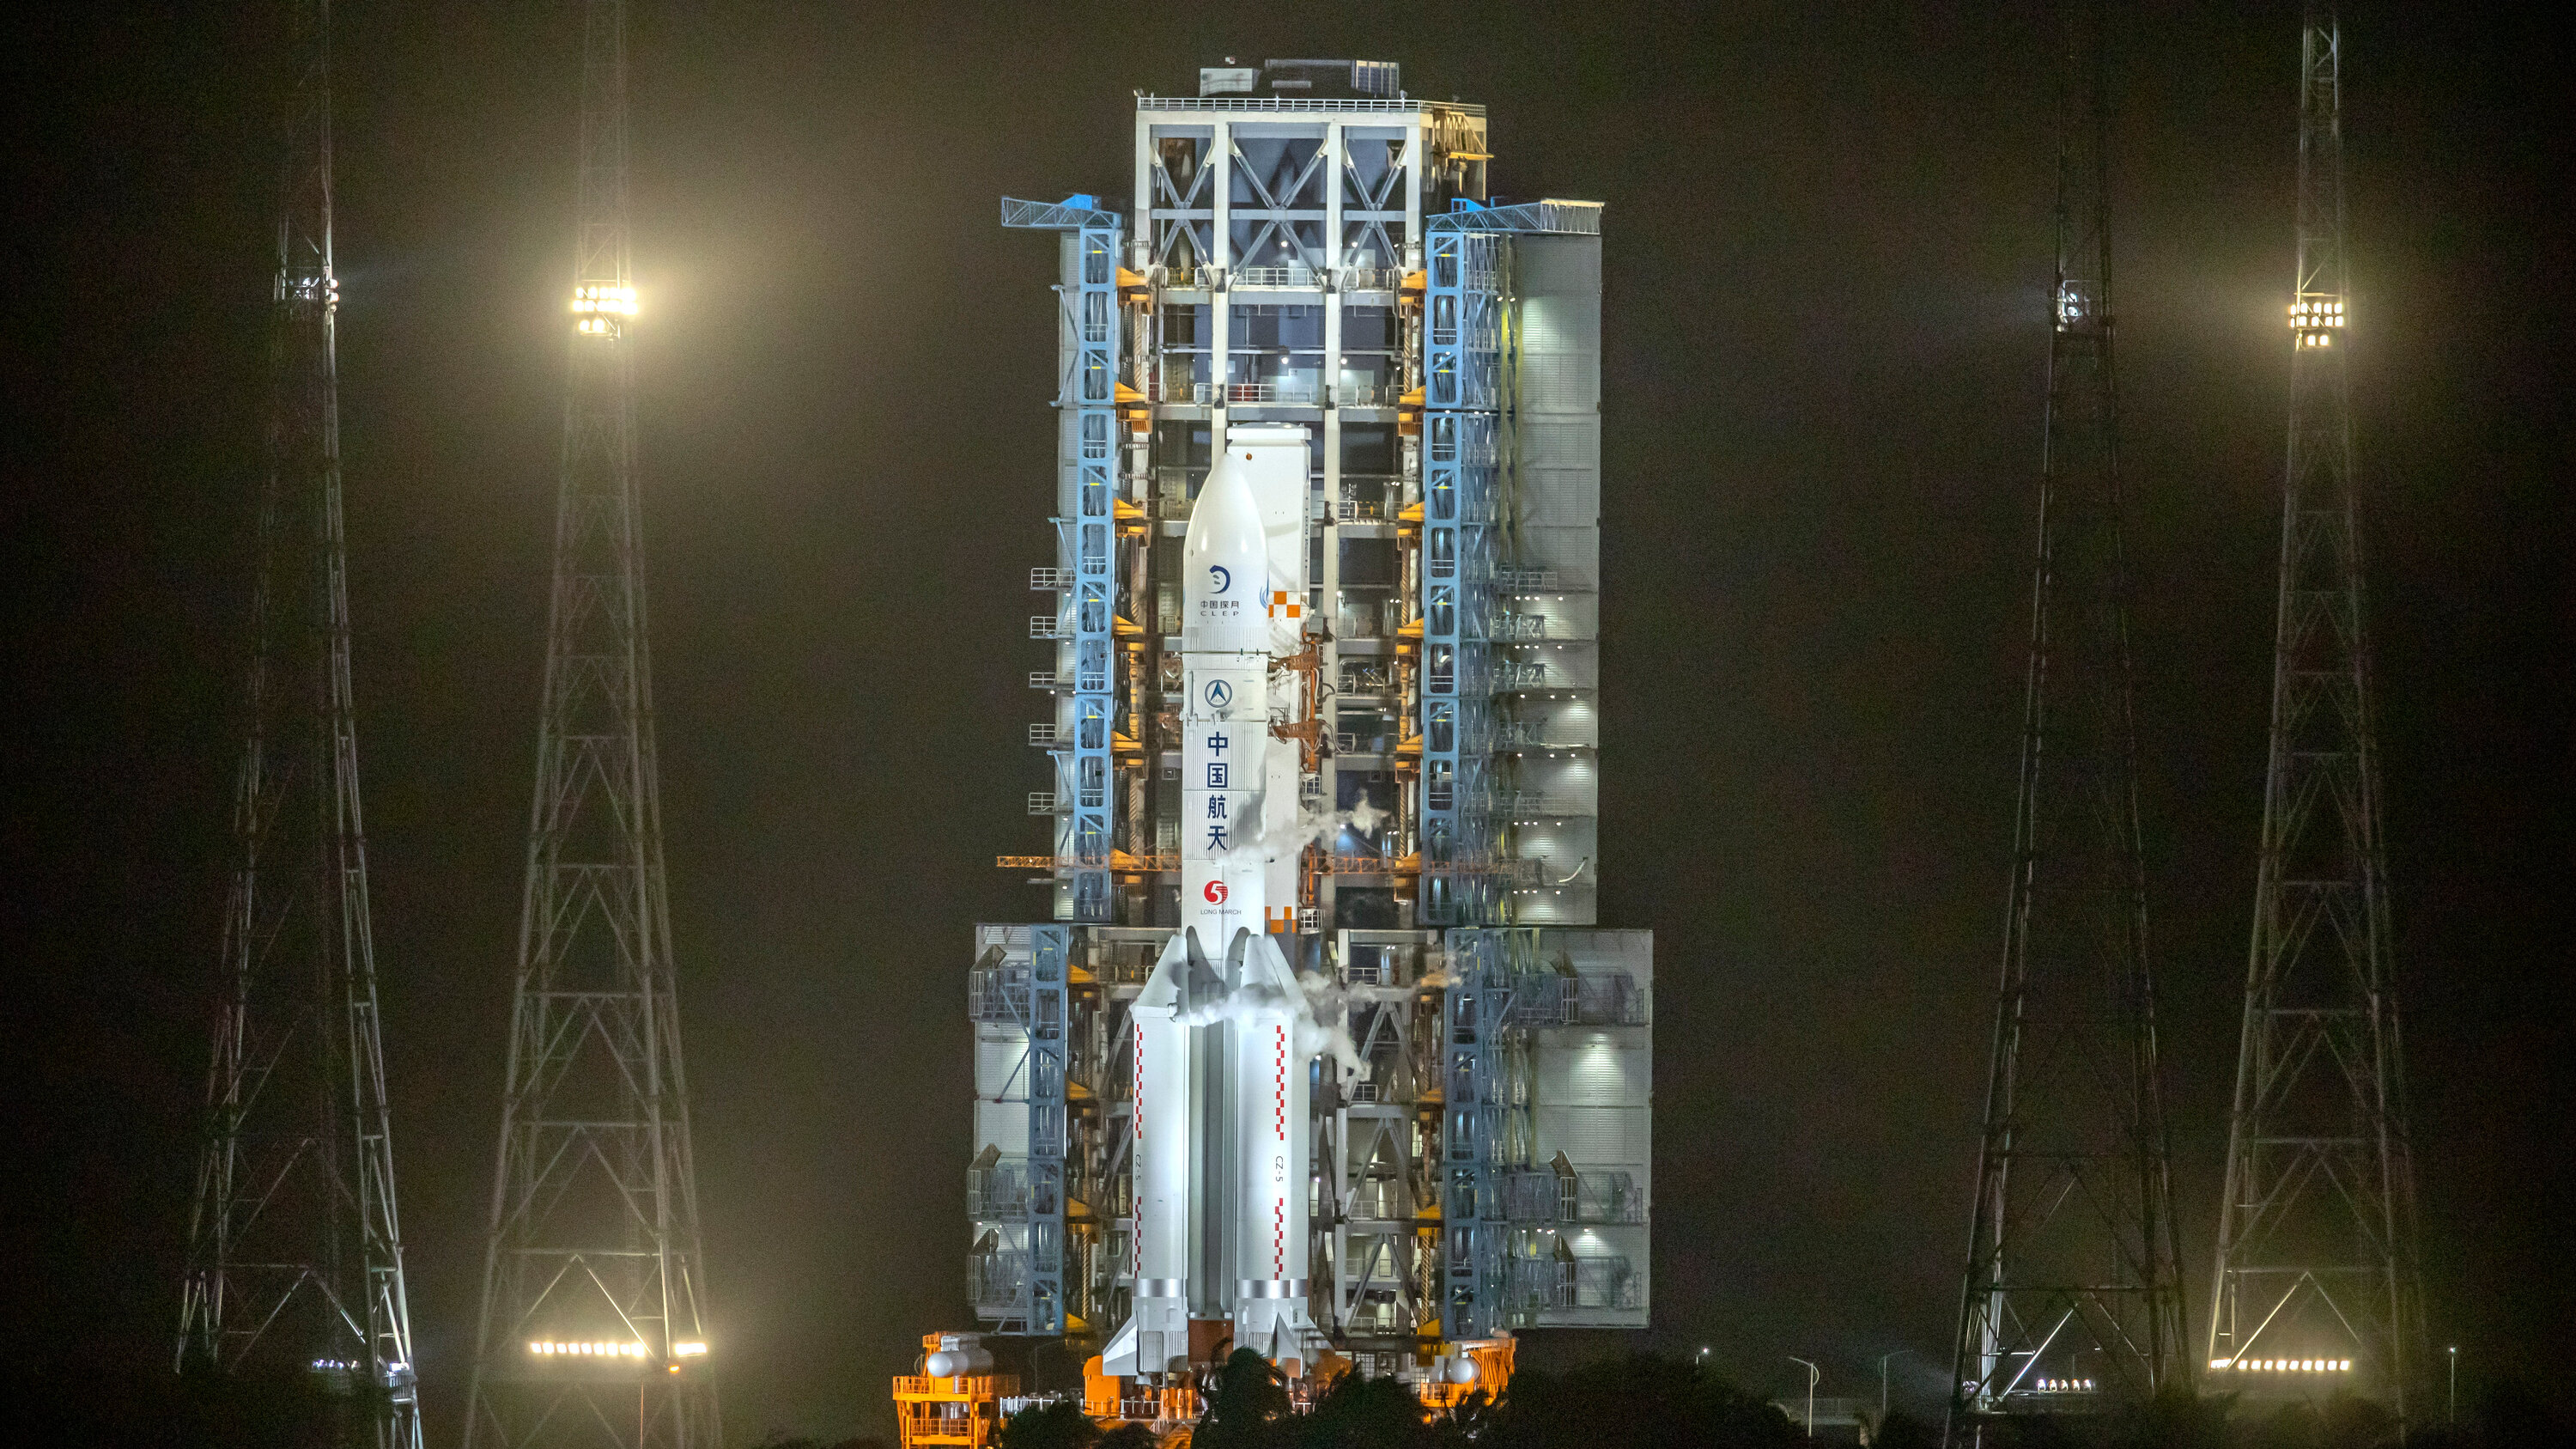
\includegraphics[width=0.8\linewidth]{CH8/Change-5.jpg}
    \end{figure}
\end{frame}

\begin{frame}{Saturn V Launch}
   \begin{figure}
       \centering
       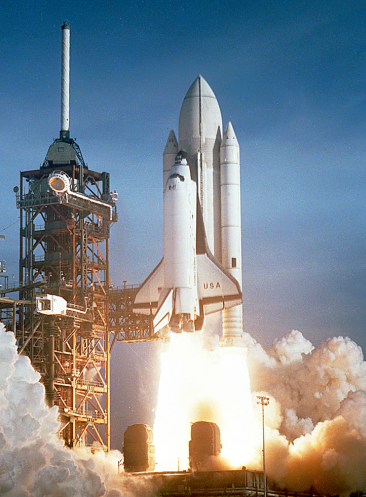
\includegraphics[width=0.4\linewidth]{CH8/Screenshot 2024-12-12 103335.png}
   \end{figure}
\end{frame}

% Title and Image Frame
\begin{frame}
\frametitle{Saturn V Launch Example}
\framesubtitle{Initial Acceleration Calculation}

% Using placeholder API for image
\begin{center}
\includegraphics[width=0.7\textwidth]{/api/placeholder/500/700}
\end{center}

\begin{block}{Saturn V Facts}
\begin{itemize}
\item Largest and most powerful rocket ever successfully operated
\item Used in Apollo moon missions
\item Height: 111 meters (363 feet)
\item Thrust at liftoff: 34.5 million newtons
\end{itemize}
\end{block}
\end{frame}

% Problem Statement Frame
\begin{frame}
\frametitle{Example 8.8: Saturn V Initial Acceleration}
\framesubtitle{Problem Setup}

\begin{block}{Given Values}
\begin{itemize}[<+->]
\item Initial mass: $m = 2.80 \times 10^6 \text{ kg}$
\item Fuel-burn rate: $\frac{\Delta m}{\Delta t} = 1.40 \times 10^4 \text{ kg/s}$
\item Exhaust velocity: $v_e = 2.40 \times 10^3 \text{ m/s}$
\end{itemize}
\end{block}

\pause
\begin{block}{Strategy}
Use rocket acceleration equation:
\[ a = \frac{v_e}{m}\frac{\Delta m}{\Delta t} - g \]
\end{block}
\end{frame}

% Solution Frame
\begin{frame}
\frametitle{Example 8.8: Solution}
\framesubtitle{Step-by-Step Calculation}

\begin{align*}
\uncover<1->{a &= \frac{v_e}{m}\frac{\Delta m}{\Delta t} - g} \\[1em]
\uncover<2->{&= \frac{2.40 \times 10^3 \text{ m/s}}{2.80 \times 10^6 \text{ kg}}}  \uncover<3->{ \times (1.40 \times 10^4 \text{ kg/s}) - 9.80 \text{ m/s}^2} \\[1em]
\uncover<4->{&= 12.0 \text{ m/s}^2 - 9.80 \text{ m/s}^2} \\[1em]
\uncover<5->{&= 2.20 \text{ m/s}^2}
\end{align*}
\end{frame}

% Discussion Frame
\begin{frame}
\frametitle{Example 8.8: Discussion}
\framesubtitle{Analysis of Results}

\begin{itemize}[<+->]
\item Initial acceleration seems small: $2.20 \text{ m/s}^2$
\item Acceleration increases as fuel burns because:
    \begin{itemize}
    \item Mass ($m$) decreases
    \item Exhaust velocity ($v_e$) remains constant
    \item Fuel burn rate ($\Delta m/\Delta t$) remains constant
    \end{itemize}

\end{itemize}

\begin{block}<5->{Key Insight}
The seemingly small initial acceleration is sufficient because it continuously increases as fuel is consumed.
\end{block}
\end{frame}

\begin{frame}{discussion time}
    
\end{frame}

% Key Concepts - Linear Momentum
\begin{frame}
\frametitle{Linear Momentum}
\begin{block}{Definition}
Linear momentum $\vec{p} = m\vec{v}$
\end{block}
\begin{itemize}
\item Vector quantity with direction same as velocity
\item SI units: kg⋅m/s
\item Proportional to both mass and velocity
\end{itemize}
\begin{equation*}
\text{Total Momentum} = \sum_i m_i\vec{v}_i
\end{equation*}
\end{frame}



% Section 8.1 Summary Frame
\begin{frame}
\frametitle{8.1 Linear Momentum and Force}
\begin{block}{Key Definition}
Linear momentum $\vec{p} = m\vec{v}$
\end{block}

\begin{itemize}
\item Linear momentum is fundamentally defined as mass × velocity
\item SI Units: kg·m/s
\item Newton's Second Law in momentum form:
\end{itemize}

\begin{equation*}
\vec{F}_{\text{net}} = \frac{\Delta \vec{p}}{\Delta t}
\end{equation*}

\begin{itemize}
\item $\vec{F}_{\text{net}}$ is net external force
\item $\Delta \vec{p}$ is change in momentum
\item $\Delta t$ is time interval
\end{itemize}
\end{frame}

% Impulse
\begin{frame}
\frametitle{Impulse}
\begin{block}{Key Equation}
$\vec{J} = \vec{F}\Delta t = \Delta \vec{p}$
\end{block}
\begin{itemize}
\item Measures change in momentum
\item Can reduce force by increasing time
\item Applications:
    \begin{itemize}
    \item Airbags
    \item Sports equipment
    \item Safety padding
    \end{itemize}
\end{itemize}
\end{frame}
\begin{frame}{Impulse Egg Drop}
    Show impulse egg drop video
\end{frame}
% Section 8.2 Summary Frame
\begin{frame}
\frametitle{8.2 Impulse}
\begin{block}{Key Concept}
Impulse equals change in momentum
\end{block}

\begin{align*}
\vec{J} &= \vec{F}_{\text{net}}\Delta t \\
&= \Delta \vec{p}
\end{align*}

\begin{itemize}
\item Impulse is the product of force and time interval
\item Forces typically vary over time
\item Area under force-time curve equals impulse
\end{itemize}
\end{frame}

% Section 8.3 Summary Frame
\begin{frame}
\frametitle{8.3 Conservation of Momentum}
\begin{block}{Conservation Principle}
In an isolated system: $\vec{p}_{\text{tot}} = \text{constant}$
\end{block}

\begin{itemize}
\item An isolated system has zero net external force
\item $\vec{p}_{\text{initial}} = \vec{p}_{\text{final}}$
\item Conserved in systems with:
    \begin{itemize}
    \item No external forces
    \item During projectile motion (horizontal direction)
    \item In particle systems
    \end{itemize}
\end{itemize}
\end{frame}

% Sections 8.4 & 8.5 Summary Frame
\begin{frame}
\frametitle{8.4 & 8.5 Collisions in One Dimension}
\begin{columns}[t]
\begin{column}{0.48\textwidth}
\textbf{Elastic Collisions}
\begin{itemize}
\item Conserves kinetic energy
\item Conserves momentum
\item Final velocities calculable from initial conditions
\end{itemize}
\end{column}

\begin{column}{0.48\textwidth}
\textbf{Inelastic Collisions}
\begin{itemize}
\item Kinetic energy not conserved
\item Momentum conserved
\item Perfectly inelastic: objects stick together
\end{itemize}
\end{column}
\end{columns}

\begin{block}{Applications}
Sports science, safety systems, particle physics
\end{block}
\end{frame}

% Section 8.6 Summary Frame
\begin{frame}
\frametitle{8.6 Two-Dimensional Collisions}

\begin{block}{Key Strategy}
Break motion into perpendicular components
\end{block}

\begin{itemize}
\item Choose x-axis parallel to incoming velocity
\item For mass 2 initially at rest:
    \begin{itemize}
    \item x-axis:
    \item $m_1v_1 = m_1v'_1\cos\theta_1 + m_2v'_2\cos\theta_2$
    \item y-axis:
    \item $0 = m_1v'_1\sin\theta_1 + m_2v'_2\sin\theta_2$
    \end{itemize}
\item Point masses cannot rotate or spin
\end{itemize}
\end{frame}
\begin{frame}{}
    \begin{figure}
        \centering
        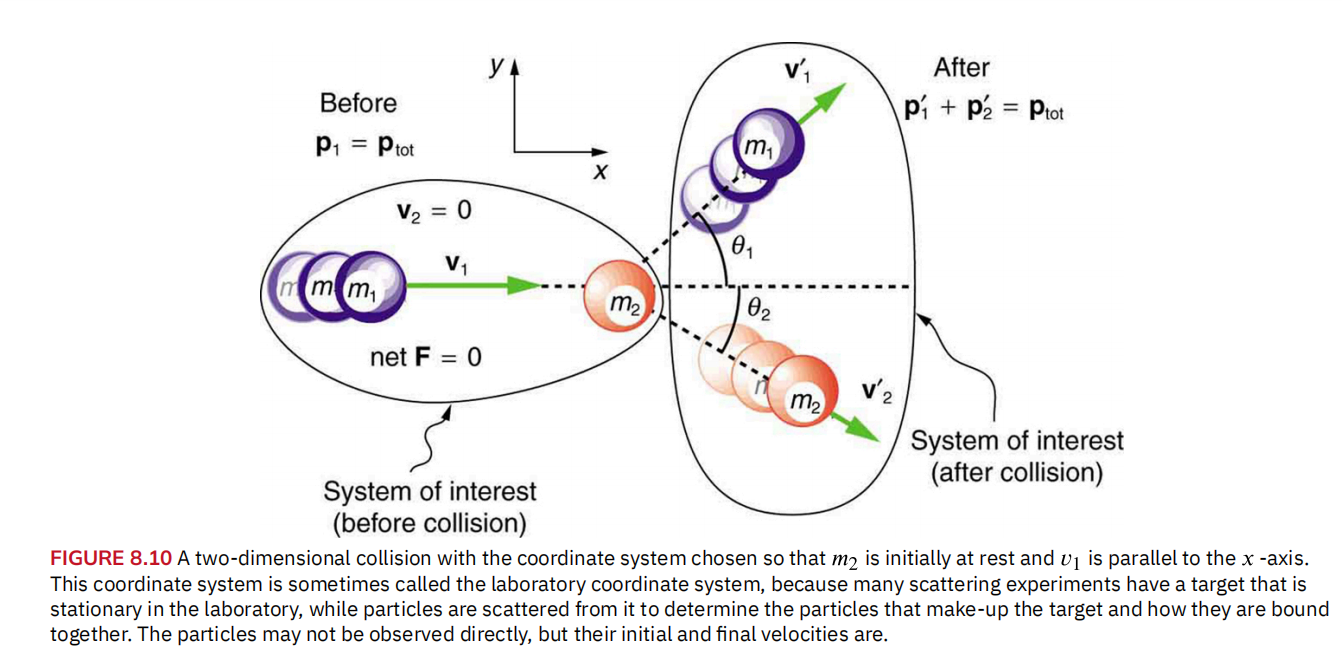
\includegraphics[width=1\linewidth]{CH8/Screenshot 2024-12-17 070905.png}
       
    \end{figure}
\end{frame}

% Section 8.7 Summary Frame
\begin{frame}
\frametitle{8.7 Rocket Propulsion}

\begin{block}{Rocket Acceleration}
$a = \frac{v_e}{m}\frac{\Delta m}{\Delta t} - g$
\end{block}

\begin{itemize}
\item Based on Newton's Third Law
\item Acceleration depends on:
    \begin{enumerate}
    \item Exhaust velocity ($v_e$)
    \item Fuel burn rate ($\Delta m/\Delta t$)
    \item Rocket mass ($m$)
    \end{enumerate}
\item Greater acceleration with:
    \begin{itemize}
    \item Higher exhaust velocity
    \item Faster fuel consumption
    \item Lower rocket mass
    \end{itemize}
\end{itemize}
\end{frame}

%%%%%%%%%%%%%%%%%%%%%%%%%%%%%%%
\iffalse
\begin{comment}
    

% I Do Example
\begin{frame}
\frametitle{Example: Elastic Collision}
\framesubtitle{I Do}
A 2.0 kg ball moving at 3.0 m/s collides elastically with a 1.0 kg ball at rest.
\begin{enumerate}
\item Conservation of momentum:
    \[ (2.0)(3.0) = 2.0v_1 + 1.0v_2 \]
\item Conservation of energy:
    \[ \frac{1}{2}(2.0)(3.0)^2 = \frac{1}{2}(2.0)v_1^2 + \frac{1}{2}(1.0)v_2^2 \]
\item Solution:
    \[ v_1 = 1.0 \text{ m/s}, v_2 = 4.0 \text{ m/s} \]
\end{enumerate}
\end{frame}
\end{comment}
%%
\fi
\end{document}